


%*****************************************
\chapter{Related Work}
\label{ch:relatedwork}
%*****************************************
\hint{This chapter should give a comprehensive overview on the related work done by other authors followed by an analysis why the existing related work is not capable of solving the problem described in the introduction (definition of the research gap!).}


%% Example for a standard figure
%%
\section{Related Work Area 1}

This section shows an example of a typical figure that can be used throughout the thesis. 
\autoref{fig:example1} visualizes the result of the \LaTeX\ code. Figures are not for decoration. They should be referenced in the text and add to the understanding of your work.


\begin{figure}[htb]
    \centering
    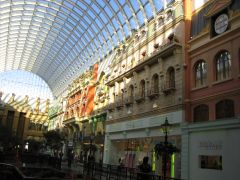
\includegraphics[width=0.5\linewidth]{gfx/example_1.jpg}
	\caption[Short Caption]{Long Caption  of Figure. Only the short caption in the squared brackets will be shown in the List of Figures.}	\label{fig:example1}
\end{figure}



%% Example for a figure with several subfigures
%%
\section{Related Work Area 2}

This section shows an example for a figure with two subfigures, shown in \autoref{fig:ex_2_3}. 
Each subfigure can be addressed individually, e.g., \autoref{fig:example_2} and \autoref{fig:example_3}.

\begin{figure}[htb]
	\centering	
	\subcaptionbox{Subcaption 1.
		\label{fig:example_2}}%
 		[.48\linewidth]{
  		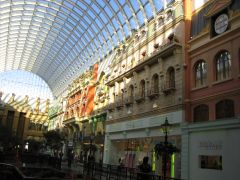
\includegraphics[width=0.35\textwidth]{gfx/example_1.jpg} 	
  	}  	
  	~
  	\subcaptionbox{Subcaption 2.
  		\label{fig:example_3}}
 		[.48\linewidth]{
  		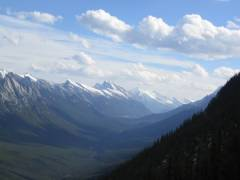
\includegraphics[width=0.35\textwidth]{gfx/example_3}  	
  	}	  
  		
	\caption{This example shows a figure with two subfigures.}
	\label{fig:ex_2_3}
\end{figure}

%%
%%
\section{Analysis of Related Work}
In the analysis of your related work, summarize your findings and define the research gap, i.e., open issues, problems, work to be done. 
The research gap builds the foundation for your own work in the following chapter(s). 